\chapter{Desarrollo}

\section{Hardware}\label{sec:hw}

El prototipo para Smart House tiene como objetivo tanto monitorear el entorno de aplicación, como controlarlo por medio de mecanismos como motores o dispositivos de iluminación, para ello está equipada con etapas de potencia de corriente alterna y directa, etapa de adquisición de datos, entre otras características que permitan cumplir con los objetivos planteados.\\ 

El prototipo fue diseñado en el software Proteus, desde el esquemático hasta la placa de circuito impreso (PCB), en la figura \ref{fig:esp32} se observa el esquematico de la tarjeta ESP32 construido en Proteus junto con su distribución de pines, además de sus conexiones correspondientes dentro de este software. El prototipo está separado en dos secciones, la etapa de potencia AC y la etapa DC, en la última, se encuentra la mayor parte de circuitos que funcionan con corriente directa.\\

\begin{figure}[H]
	\centering
	\caption{ESP32 creado en proteus [Imagen Propia]}
	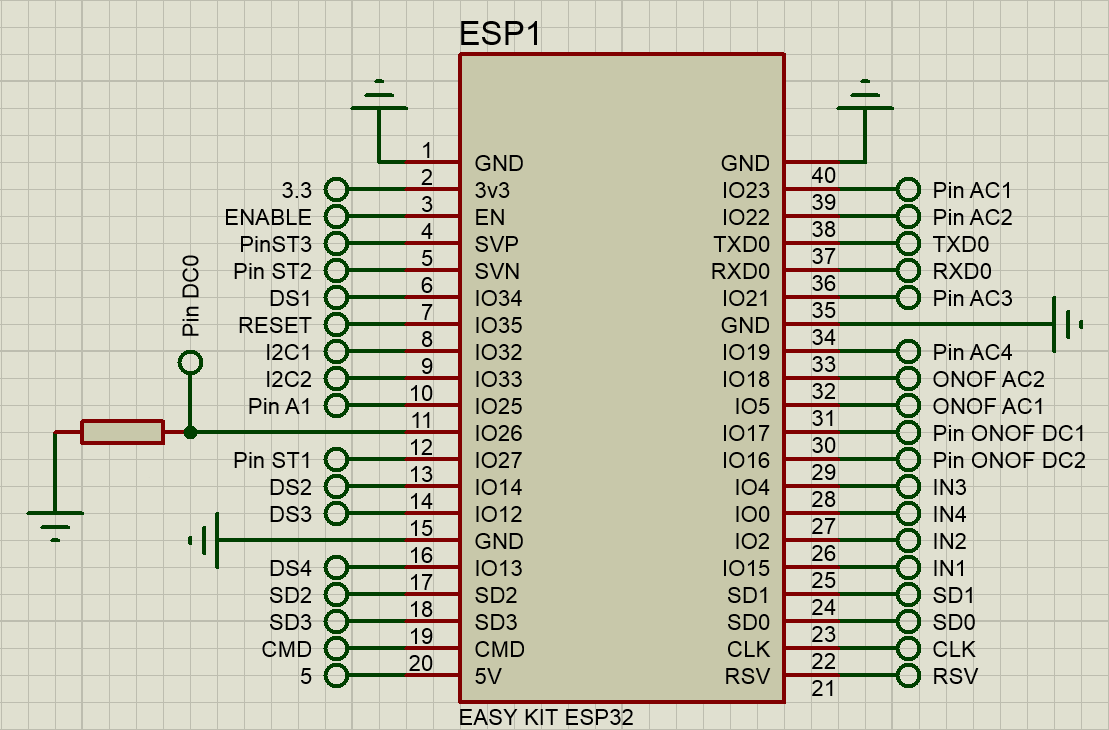
\includegraphics[width=0.5\linewidth]{Imagenes/ESP32}	
	\label{fig:esp32}
\end{figure}

En los siguientes ítems se resaltaran las características más importantes que lleva el circuito:\\

	\subsection{Alimentacion:}
	
	\subsubsection{Corriente alterna (AC):}
		El prototipo recibe el voltaje directamente de la red eléctrica a la cual está conectado el entorno de aplicación, el cual está pensado para una habitación dentro de una Smart House; en el caso de Colombia, la red doméstica comúnmente otorga 110V AC, los cuales son regulados para el funcionamiento adecuado del prototipo,  como la etapa de potencia AC y el detector de cruce por cero para sincronizar la tarjeta a dicha red eléctrica.\\
		
	\subsubsection{Corriente directa (DC):}
		Para la alimentación DC del circuito se hace uso de un conversor AC-DC que regula el voltaje de la red eléctrica a 12V DC, con los cuales se manejara la etapa de potencia DC, además de ser usados por dos modulos conversores DC-DC, mostrados en la figura \ref{fig:DCDC}, ambos con entradas de 12V DC y con salidas a los niveles lógicos comunes, tales como 5V y 3.3V, empleados para alimentar dispositivos como opto acopladores,  transistores BJT o relevadores con activación de 5V, así como también la tarjeta de 	prototipo ESP32.\\
		
		Cabe resaltar que la tarjeta permite una entrada externa de 12VDC a 5A si se desean controlar cargas a un máximo de 50W.\\
			
		\begin{figure}[H]
			\centering
			\caption{Modulo conversor DC-DC \cite{DCDC}}
			\label{fig:DCDC}
			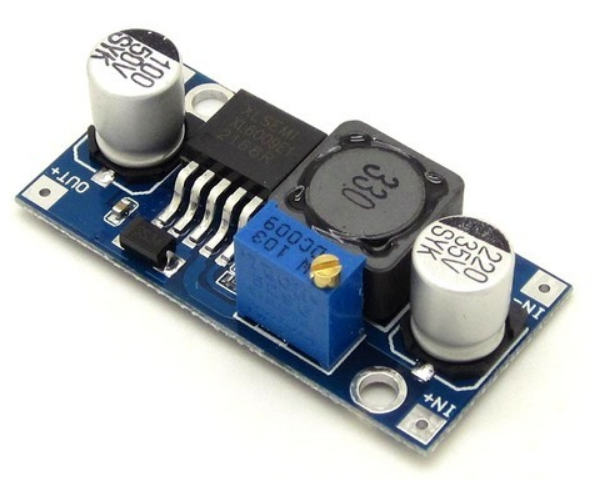
\includegraphics[width=0.5\linewidth]{Imagenes/DCDC}
		\end{figure}
	
	\subsection{Entradas:}
	\subsubsection{Sensores:}
		El prototipo viene equipado con una etapa de adquisición de datos con capacidad entre 7 a 134 sensores, pues está equipado con entrada I2C, ampliando la capacidad de dispositivos conectados, lo cual también permitiría adicionar tareas más específicas en escenarios que lo requieran.\\
		
		Para realizar pruebas del prototipo, se hacen uso de 5 sensores para medir magnitudes y situaciones en el entorno tal como calidad del aire, temperatura y humedad, luz visible, movimiento y presencia de lluvia, debido a que estas magnitudes o estados se encuentran en casi cualquier entorno. Para esto, teniendo en cuenta que el ESP32 funciona en voltajes lógicos de 3.3V, se tienen 4 entradas de sensores directamente conectados a los pines de la tarjeta, con la capacidad de cambiar el voltaje de alimentación para 3 de ellos, tal como se muestra en la figura \ref{fig:SVS}, pues en el mercado se encuentran sensores que manejan voltajes de alimentación ya se de 3.3V o 5V, mientras que la cuarta entrada se encuentra alimentada con 5V, ya que tiene un uso específico en las pruebas para el sensor de calidad de aire, dicha entrada viene acondicionada con un diodo zener en contraposición, para evitar que la tarjeta ESP32 tenga un voltaje de entrada superior a 3.3V, como se observa en la figura \ref{fig:S1Aire}.\\
		
		Las tres entradas para sensores de estado (ST1, ST2, ST3), a diferencia de las demás, se encuentran conectadas a pines de la tarjeta que no presentan resistencia de pull down por software, por ello se agrega dicha resistencia al sistema, tal como se observa en la figura \ref{fig:ST}.\\
		
		\begin{figure}[H]
			\centering
			\caption{Entrada de sensores[Imagen Propia]}
			\label{fig:SVS}
			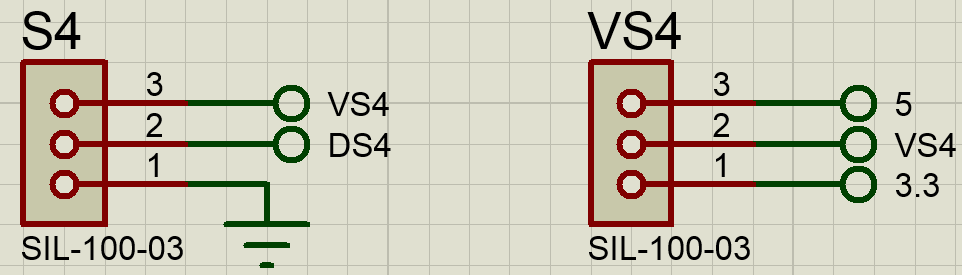
\includegraphics[width=0.7\linewidth]{Imagenes/SVS}
		\end{figure}
	
		\begin{figure}[H]
			\centering
			\caption{Entrada para sensor de calidad de aire[Imagen Propia]}
			\label{fig:S1Aire}
			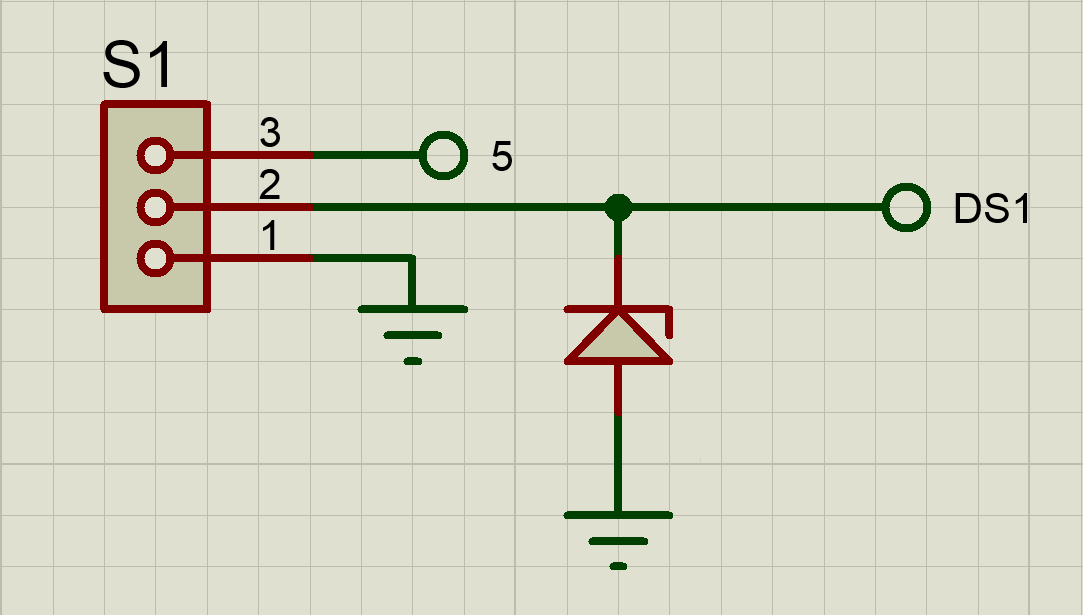
\includegraphics[width=0.6\linewidth]{Imagenes/S1Aire}
		\end{figure}
	
		\begin{figure}[H]
			\centering
			\caption{Entrada para sensores con resistencia de pull down[Imagen Propia]}
			\label{fig:ST}
			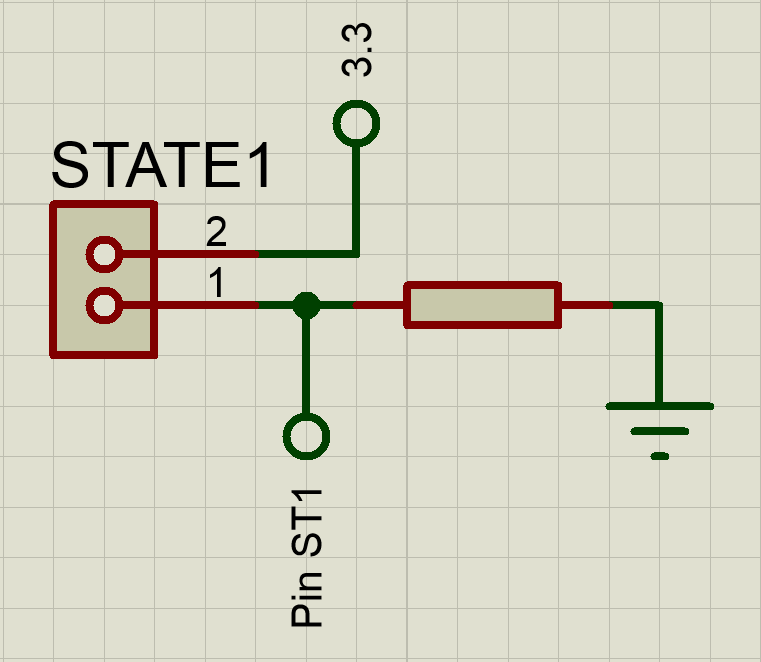
\includegraphics[width=0.5\linewidth]{Imagenes/ST}
		\end{figure}		
	
	\subsubsection{Calibración de audio:}
		Para calibrar la salida audible se hace uso de una resistencia variable (Potenciometro), el cual permite regular el voltaje de entrada al circuito de amplificación, mostrado en la figura \ref{fig:AUD} y será descrito en el presente capitulo en la sección de salidas del hardware.\\
		
	\subsubsection{Botón enable:}
		Presionando el botón enable se reinicia la tarjeta ESP32, junto con su firmware.\\
		
	\subsubsection{Botón reset:}
		Presionando el botón reset se reinician las credenciales ingresadas para la conexión correcta del ESP32 a la red wifi.\\
		
	\subsection{Salidas:}
	\subsubsection{Etapa de potencia AC:}
		La etapa de potencia AC del prototipo, está diseñada para una potencia de 2000W en un total de seis cargas, cuatro de ellas cuentan con un circuito para el control por ángulo de fase, como se observa en la figura \ref{fig:CAC1}, con una capacidad individual de 500W, gracias a el TRIAC de potencia BTA26600, mostrado en la figura \ref{fig:TRIAC}, el cual soporta una corriente máxima de 25A; para proteger el ESP32, se hizo uso de optoacopladores MOC3021, debido a su capacidad para aislar circuitos de forma óptica.\\
		
		\begin{figure}[H]
			\centering
			\caption{Control por angulo de fase [Imagen Propia]}
			\label{fig:CAC1}
			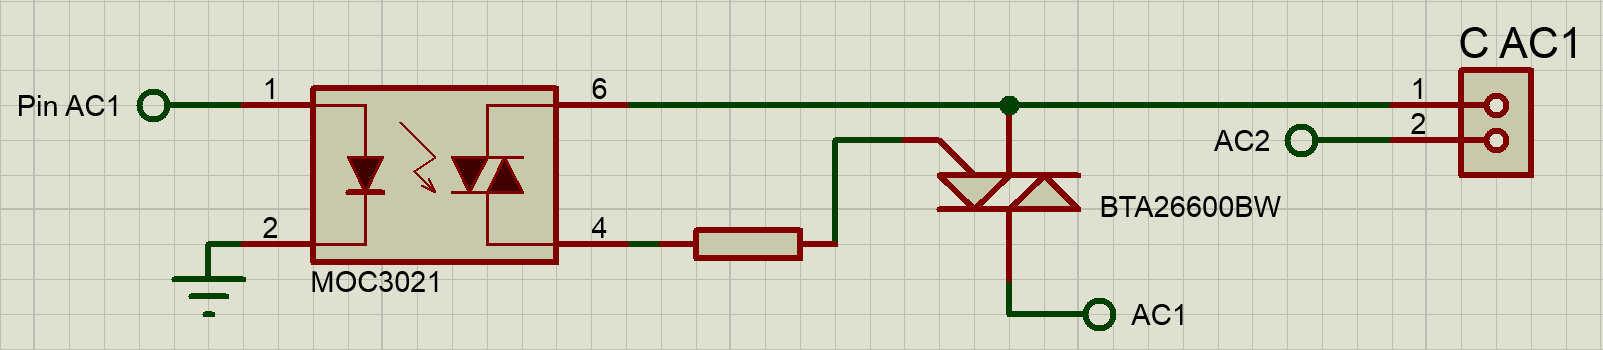
\includegraphics[width=0.8\linewidth]{Imagenes/CAC1}
		\end{figure}
	
		\begin{figure}[H]
			\centering
			\caption{Triac BTA26600 \cite{TRIAC}}
			\label{fig:TRIAC}
			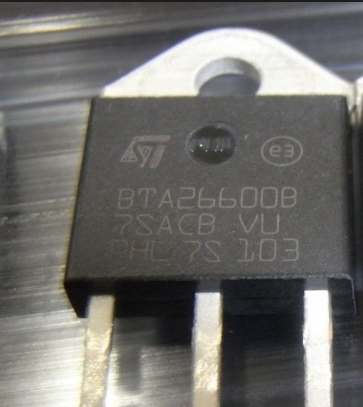
\includegraphics[width=0.35\linewidth]{Imagenes/TRIAC}
		\end{figure}
	
		Las dos cargas restantes corresponden a un sistema de encendido y apagado, cuyo funcionamiento se basa en un relevador SRA-05VDC-CL activado a 5V por medio de un transistor BJT como switch, gracias a este relevador, la salida tiene capacidad para cargas de 200W cada una, en la figura \ref{fig:ONOFAC} se observa el circuito diseñado en proteus. Para proteger el ESP32 el prototipo se vale del relevador, puesto que presenta un aislamiento magnético por la naturaleza de su funcionamiento.\\
	
		\begin{figure}[H]
			\centering
			\caption{Interruptor para cargas AC [Imagen Propia]}
			\label{fig:ONOFAC}
			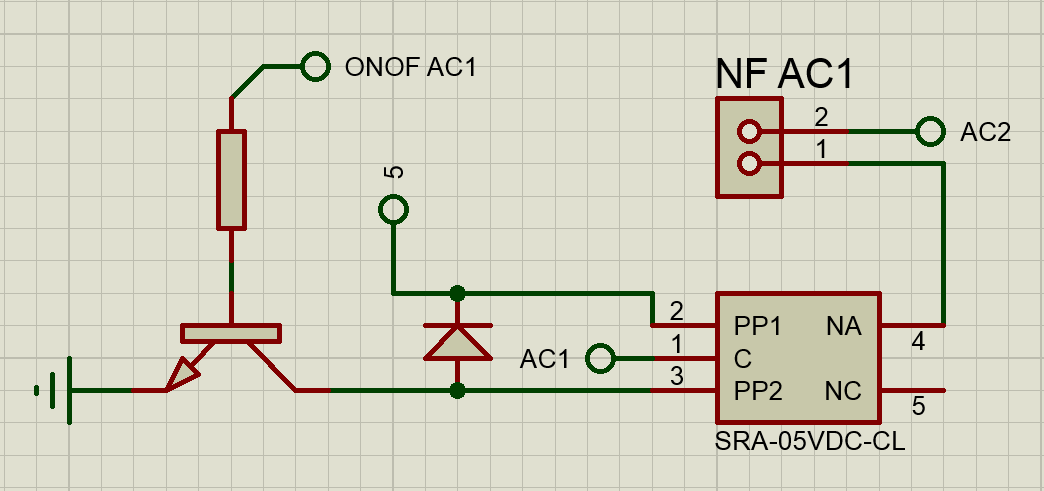
\includegraphics[width=0.7\linewidth]{Imagenes/ONOFAC}
		\end{figure}
	
		Dentro de la etapa AC se encuentra el detector de cruce por cero, el cual se vale de un fototransistor 4N25, debido a su alta capacidad de aislamiento, soportando más de 2500VAC, tomando la onda rectificada completa y pasándola a un nivel lógico de 3.3V, esta parte del circuito se observa en la figura \ref{fig:DC01}; para que la señal sea más confiable se hace uso de un Schmitt-Trigger CD40106 mostrado en la figura \ref{fig:DC02}, valiéndose de la histéresis de voltaje para garantizar que su señal de salida sea poco susceptible al ruido \cite{DC0}.\\
		
		\begin{figure}[H]
			\centering
			\caption{Detector de cruce por cero [Imagen Propia]}
			\label{fig:DC01}
			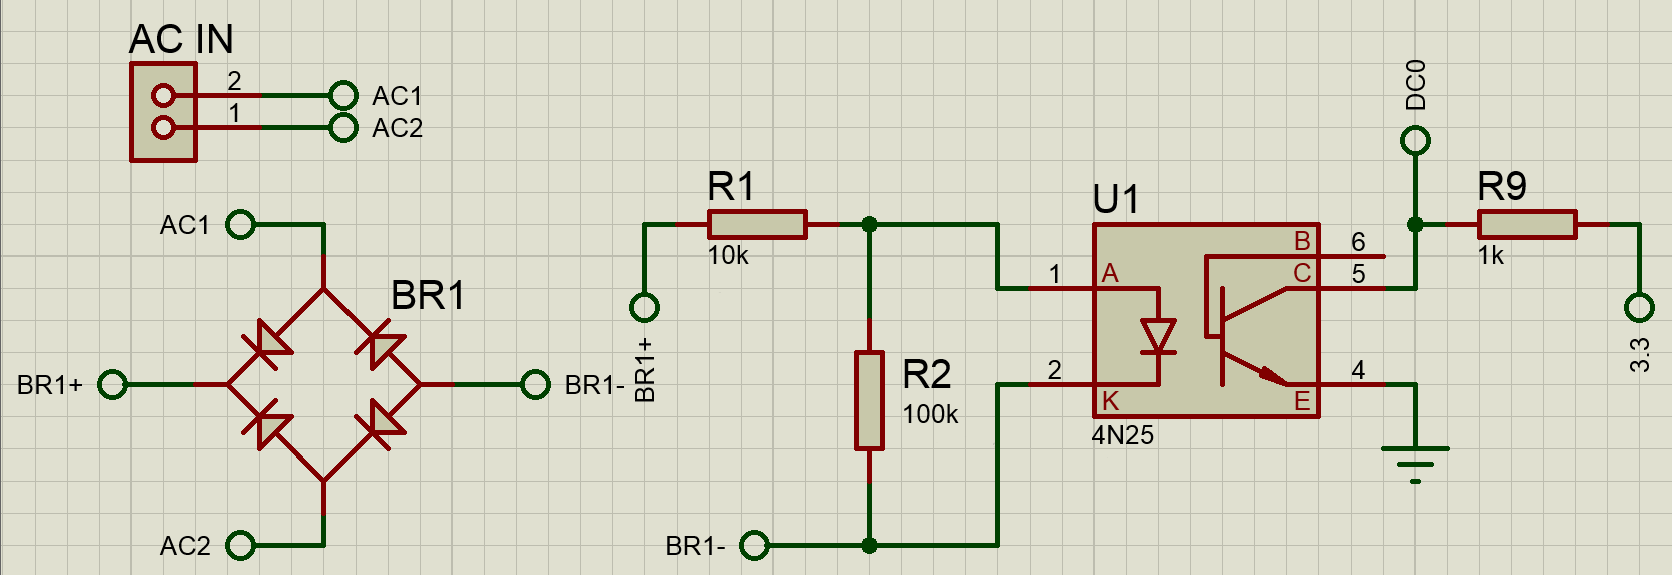
\includegraphics[width=0.85\linewidth]{Imagenes/DC01}
		\end{figure}
	
		\begin{figure}[H]
			\centering
			\caption{Schmitt trigger para el detector de cruce por cero [Imagen Propia]}
			\label{fig:DC02}
			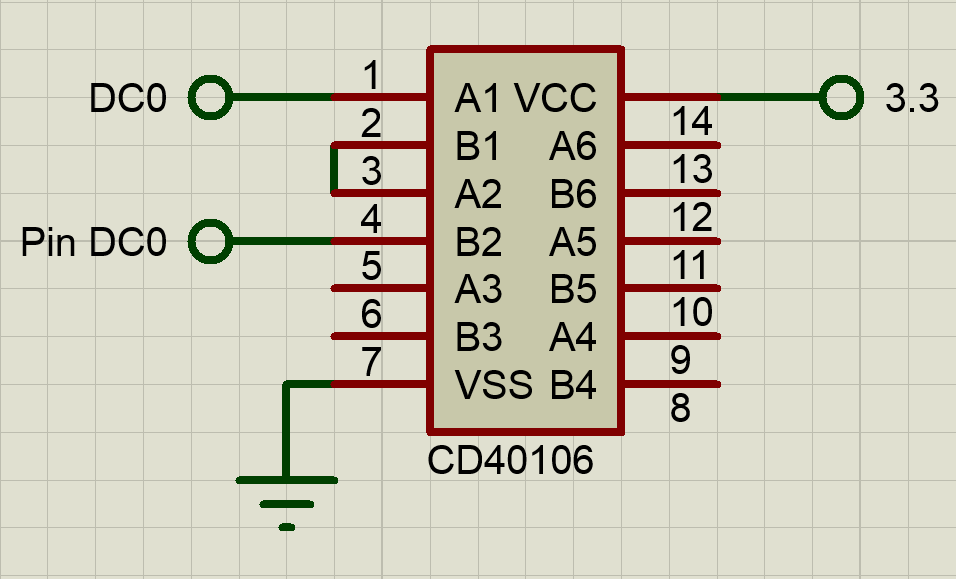
\includegraphics[width=0.5\linewidth]{Imagenes/DC02}
		\end{figure}
	
	\subsubsection{Etapa DC:}
		La etapa DC cuenta con cuatro salidas de control diseñadas para cargas de 12V, de las cuales, dos de ellas están diseñadas con enfoque a motores, puesto que está equipada con control de velocidad a base de PWM e inversión de giro con un puente h usando transistores mosfet IRLZ44N; este puente h está controlado por un circuito integrado L293D, que garantiza un voltaje Vgs adecuado para la correcta activación del los transistores del puente h; este circuito se muestra en la figura \ref{fig:L293D} y \ref{fig:CDC}.\cite{IRL}.\\
		
		Las dos salidas restantes también cuentan con mosfet IRLZ44N, y su control también es a base de PWM, mas no permite hacer inversión de giro, por lo cual se enfoca a dispositivos como lámparas LEDs, el diseño en proteus se muestra en la figura \ref{fig:ONOFDC}.\\
		
		\begin{figure}[H]
			\centering
			\caption{Integrado L293D [Imagen Propia]}
			\label{fig:L293D}
			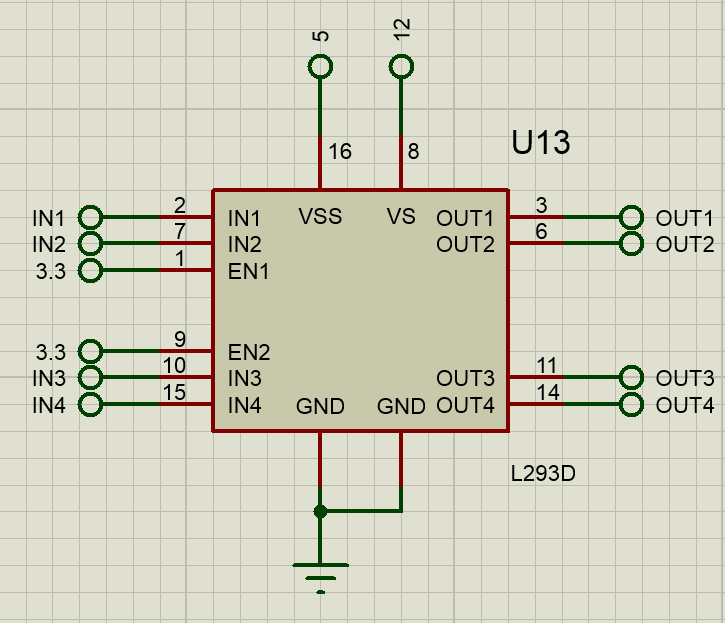
\includegraphics[width=0.5\linewidth]{Imagenes/L293D}
		\end{figure}
		
		\begin{figure}[H]
			\centering
			\caption{Puente h para control de motores DC [Imagen Propia]}
			\label{fig:CDC}
			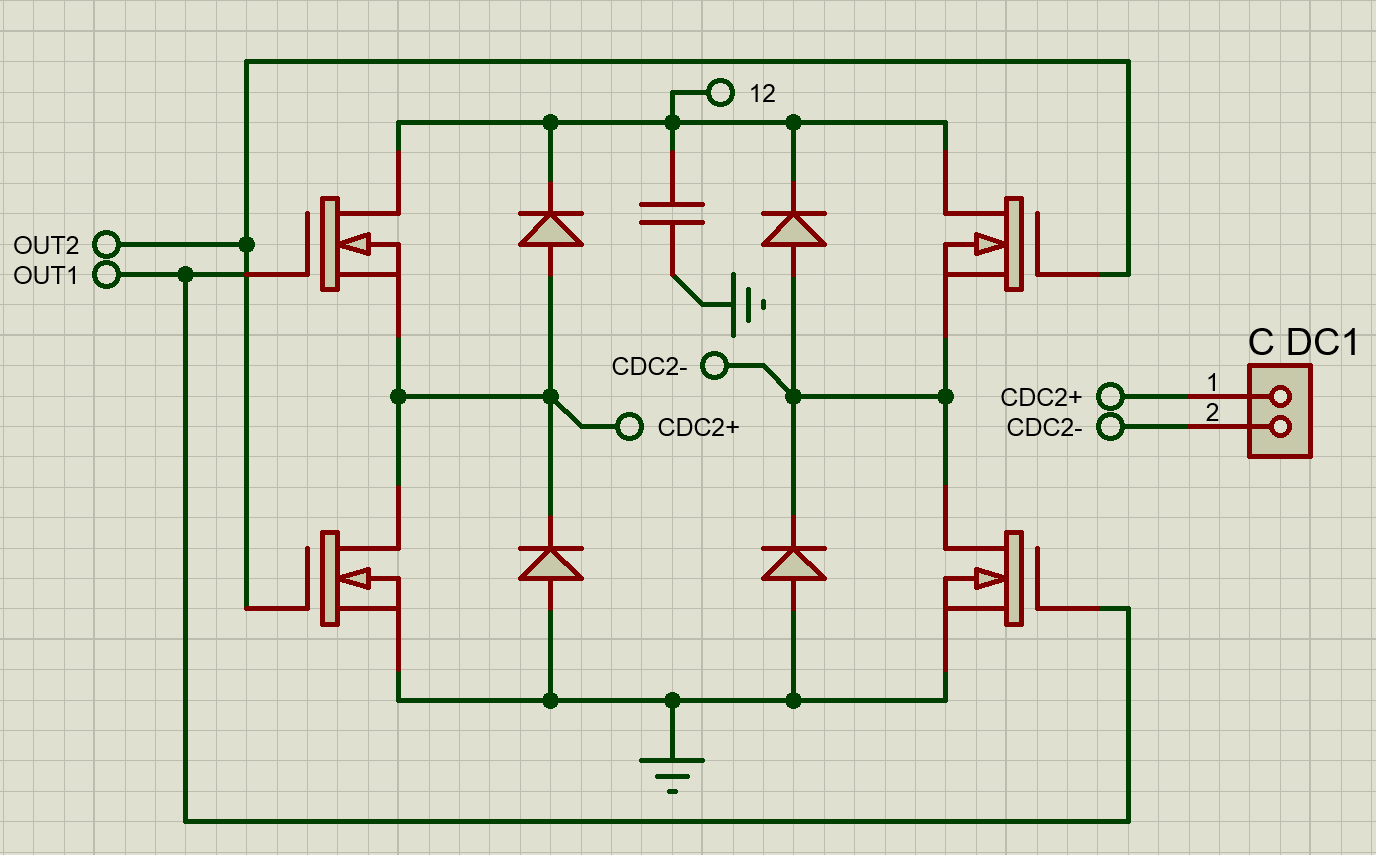
\includegraphics[width=0.7\linewidth]{Imagenes/CDC}
		\end{figure}
	
		\begin{figure}[H]
			\centering
			\caption{Control para cargas DC [Imagen Propia]}
			\label{fig:ONOFDC}
			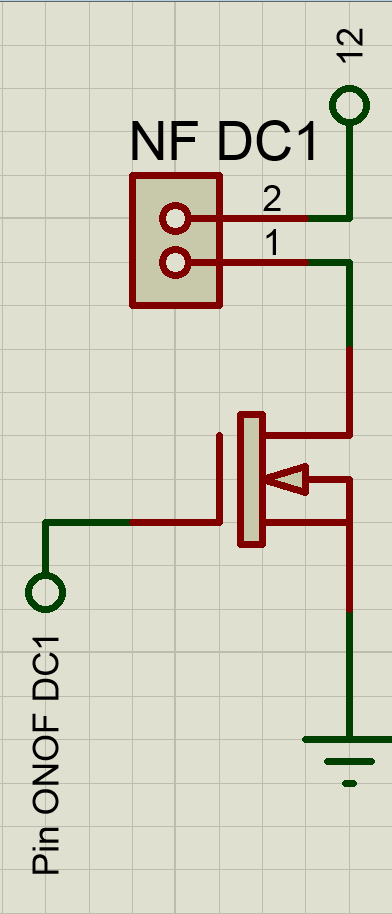
\includegraphics[width=0.25\linewidth]{Imagenes/ONOFDC}
		\end{figure}
	
	\subsubsection{Salida audible:}
		La salida audible está diseñada para emitir desde sonidos a una sola frecuencia, o sonido mono estéreo, caso dado cuando se activa una regla programada desde la aplicación web, enfocada a las cargas de encendido y apagado, tanto de la etapa de potencia AC como la etapa DC; el sonido emitido por el prototipo corresponde a una voz con tonalidad femenina, pronunciando el estado en el cual se configura la carga según la regla (ya sea encendido, o apagado).\\
		
		El circuito utilizado para la salida audible está basado en el amplificador de audio LM386, implementando el circuito típico de aplicación ilustrado en su datasheet  \cite{LM386}, en la figura \ref{fig:AUD} se observa este circuito implementado en proteus.\\
		
		Como se mencionó anteriormente, el circuito presenta un potenciómetro a la entrada para calibrar el voltaje de esta, con el fin de no saturar la entrada para que el sonido a la salida sea lo mas fiel posible.
				
		\begin{figure}[H]
			\centering
			\caption{Circuito tipico para el LM386 [Imagen Propia]}
			\label{fig:AUD}
			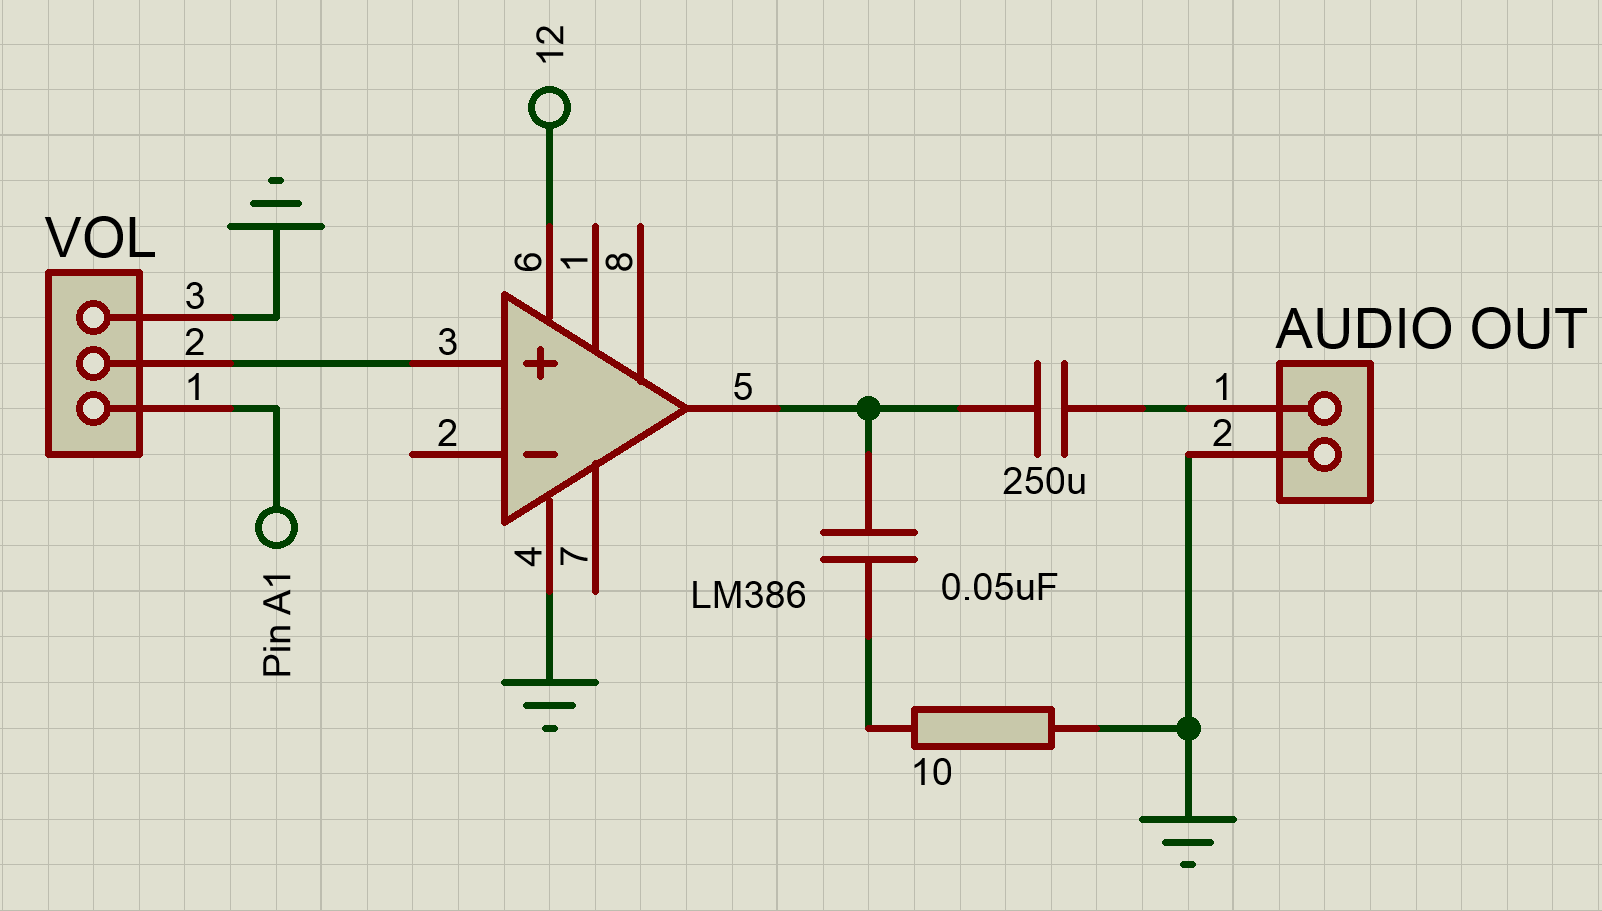
\includegraphics[width=0.7\linewidth]{Imagenes/AUD}
		\end{figure}		
				
\section{Firmware}

El firmware se desarrolla sobre el framework o SDK oficial de Espressif Systems, ESP-IDF el cual posee una documentación \cite{ES} muy útil a la hora de utilizar las diferentes APIs que este posee; para el desarrollo de la aplicación es necesario contar con los diferentes requisitos tal como se observa en la figura \ref{fig:what-you-need}. Este firmware incluye un kernel de tiempo real llamado FreeRTOS, el cual da soporte al manejo de los diferentes recursos del sistema; Al ser este  un RTOS, las funciones se definen mediante las tareas, entonces para cada funcionalidad de la tarjeta o grupo de funcionalidades se desarrolla una o varias tareas para que realicen las acciones adecuadas, por ejemplo, en el caso de los sensores, cada uno tiene una tarea para lectura y para gestión de datos, así como también ocurre de manera similar  con las diferentes salidas de la tarjeta, pues cuentan con tareas para la gestión de encendido y apagado así como también para el control de cargas, ya sea por ángulo de fase o PWM.\\

\begin{figure}[H]
	\centering
	\caption{ESP-IDF \cite{ES}}
	\label{fig:what-you-need}
	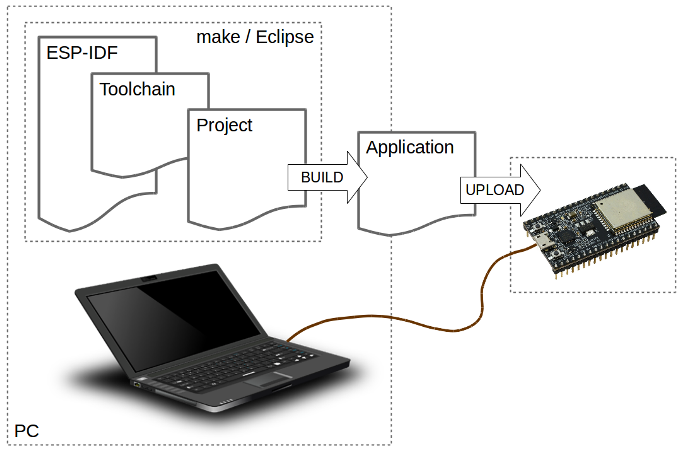
\includegraphics[width=0.5\linewidth]{Imagenes/what-you-need}
\end{figure}


Sobre el firmware se desarrollan los siguientes temas:

\paragraph{Tareas:}

se ejecutan constantemente en el sistema operativo, realizando diferentes funciones para lectura, escritura y control.

\paragraph{GPIO:}

el ESP-WROOM-32 posee diferentes GPIO, los cuales se usan para leer o escribir señales digitales, en cuanto a los sensores se pueden enviar señales para iniciar su lectura o simplemente tener el pin en modo entrada y leerlo cada cierto intervalo de tiempo para generar los datos de lectura, o en modo salida para el control de los diferentes dispositivos que se han desarrollado en el hardware.

\paragraph{ADC,DAC:}

los ADC se usan para leer los datos de algunos sensores que proporcionan datos analógicos, por este motivo se hace la conversión de la señal analógica a un valor digital dentro de la tarjeta, para luego identificar el valor de la lectura del sensor. Los DAC se usan para realizar la operación contraria, teniendo valores digitales convertirlos a un valor analógico por ejemplo para generar audios o diferentes señales a partir del software.

\paragraph{Consola:}

para realizar diferentes pruebas directamente desde la tarjeta, se usa la opción de la consola, la cual se comunica por medio del puerto serie, para esto se crean las funciones y los comandos que estaran disponibles; Algunos comandos disponibles son \textit{http}, para realizar las peticiones http manualmente y observar su respuesta, \textit{pin} para realizar la prueba de un pin digital como entrada o salida, \textit{help} para observar la lista de comandos, entre otros.

\paragraph{HTTP Request:}

las peticiones HTTP son indispensables en estas aplicaciones del campo IOT, por este motivo en el desarrollo del firmware se usan las librerias pertinentes para realizar peticiones y además leer las respuestas de estas desde el servidor, ya que este es el medio de comunicación tarjeta-servidor.

\paragraph{Hora de Red:}

se obtiene la hora mediante el protocolo simple de tiempo de red (SNTP), este resulta de gran utilidad para la sincronización de los relojes de los sistemas informáticos. Se mantiene actualizada para realizar diferentes acciones respecto a esta.

\paragraph{Timers:}

la tarjeta posee dos grupos de timers, que cuenta cada uno con dos timers, un timer lo usa el sistema operativo, otro es configurado para realizar el control de potencia AC por ángulo de fase, para tener la sincronía necesaria con la señal de la red eléctrica.

\paragraph{I2C:}

el protocolo I2C se activa por medio de la instalación del driver en algún par de pines GPIO disponibles en la tarjeta. Se configura e inicia y posteriormente se crea una tarea la cuál se encarga de solicitar y leer los datos de los diferentes sensores conectados a este.

\paragraph{PWM:}

se ha mencionado anteriormente que para controlar las cargas DC se usa una salida PWM, el esp32 proporciona esta funcionalidad en algunos de sus pines, para su uso se configura y asignan los valores de funcionamiento.

\paragraph{Interrupciones:}

las interrupciones se usan para no gastar recursos en un monitoreo constante de las entradas, solo cuando exista un cambio de nivel en la entrada el dispositivo desencadena una serie de instrucciones relacionas al tipo de interrupción y a diferentes funciones creadas para esta, la interrupción se usa por medio de los diferentes pines propuestos para esto en el hardware.

\section{Software}

En esta sección se desarrolla una aplicación web, la cual se encarga de hacer la gestión entre el usuario y la tarjeta. De este modo, se usa un patrón de arquitectura Modelo-Vista-Controlador (MVC). Este modelo es realmente útil ya que separa la lógica de negocio de la interfaz de usuario, incrementando la reutilización y flexibilidad, además la escalabilidad de ambos aspectos por separado, dicho esto la aplicación cuenta con diferentes modelos, controladores y vistas \cite{MVC1}. La función de cada parte de esta arquitectura se puede observar en la figura \ref{fig:mvc}.\\

\begin{figure}[H]
	\centering
	\caption{Modelo-Vista-Controlador}
	\label{fig:mvc}
	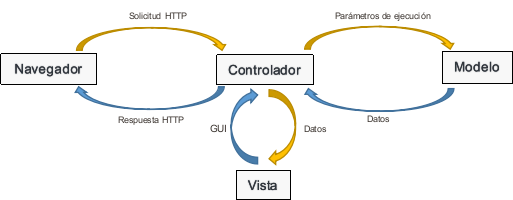
\includegraphics[width=0.7\linewidth]{Imagenes/MVC}
\end{figure}


Su funcionamiento es el siguiente, primero el usuario realiza alguna acción en la interfaz (por ejemplo, presiona un botón, un enlace, etc), luego el controlador recibe (por parte de los objetos de la interfaz-vista) la notificación de la acción solicitada por el usuario. El controlador gestiona el evento que llega. Luego el controlador accede al modelo, actualizándolo, posiblemente modificándolo de forma adecuada a la acción solicitada por el usuario (por ejemplo, el controlador actualiza los datos del perfil del usuario) y después la interfaz de usuario espera nuevas interacciones del usuario, comenzando el ciclo nuevamente \cite{MVC2}.\\

Este patrón de diseño se usa en la programación orientada a objetos, por lo tanto se realiza la aplicación en el lenguaje de programación PHP, ya que es realmente útil para realizar la gestión de peticiones y envíos de formularios en dicha aplicación, además de que es importante también la gestión de las bases de datos de la aplicación, por este motivo se utiliza un framework basado en este lenguaje y esta arquitectura, el cual realiza diferentes trabajos en cuanto a la parte de la arquitectura. Para gestionar las diferentes partes de la aplicación, en este caso se usa el framework Laravel, el cual como se menciona anteriormente está orientado a facilitar las tareas comunes de la mayoría de proyectos web que utilizan HTML5 y PHP.\\

Además, con este framework se hace uso de un ORM (Mapeo Objeto-Relacional) llamado Eloquent. Esta es una forma de mapear los datos que se encuentran en la base de datos a objetos de PHP y viceversa, esto facilita el uso de diferentes gestores de bases de datos como MySQL, SQLite, entre otras, ya que todas las consultas estan en PHP y el ORM ya se encarga del mapeo a los comandos SQL como se observa en la figura \ref{fig:orm}. Eloquent usa los modelos para enviar y recibir información de la base de datos\cite{Eloq}.\\

\begin{figure}[H]
	\centering
	\caption[ORM]{ORM [Imagen Propia]}
	\label{fig:orm}
	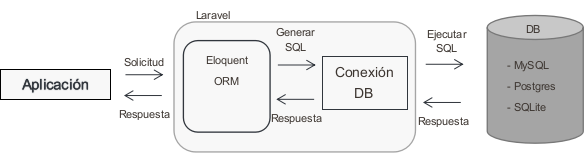
\includegraphics[width=0.7\linewidth]{Imagenes/ORM}
\end{figure}

\section{Prueba Beta}

Esta prueba se desarrolla en el entorno del cliente o usuario, arrojando resultados sobre las funcionalidades provistas para el software, además de dar la aceptación por parte del cliente si el producto funciona de manera adecuada o esperada \cite{PB}. Los diferentes casos de prueba a realizar son los siguientes:

\paragraph{Prueba de conectividad de la tarjeta:} en la cual se califica la forma en que el cliente conecta la tarjeta SmartHouse a Internet por medio de Wi-Fi.

\paragraph{Prueba de la Aplicación Web:} en la cual se evalúan diferentes aspectos y la mas extensa, ya que se evalúa el inicio de sesión, el monitoreo y control de todos los dispositivos que se encuentra conectados en tarjeta SmartHouse.